\refstepcounter{section}
\section*{Lecture 13: Landau Theory for Phase Transition: III}
\addcontentsline{toc}{section}{Lecture 13: Landau Theory for Phase Transition: III}
In this lecture, we focus on how the order parameter changes and the emergence of interesting phenomenon like hysterisis, for the $m^3$ and $m^6$ Landau theory.
\subsection{Order Parameter Flow for $m^3$}
Consider the previous case of $\SL$ with $m^3$ term. We can change this to a one-parameter problem, following a transformation. We want to keep the one parameter $r$ associated with $a_2$, since this is where the temperature dependence is there. The other parameters need to be scaled somehow. If we say, $a_3 = c a_4$, then we obtain 

$$\SL = a_4\qty(\frac{a_2}{2a_4}(T-T_c) m^2 -\frac{1}{3} c m^3+\frac{1}{4} m^4)$$
If we now define the scaling $m=cu$ then we obtain,
$$\SL = a_4\qty(\frac{a_2}{2a_4}(T-T_c) c^2 u^2 -\frac{1}{3} c^4 u^3+\frac{1}{4} c^4 u^4)$$
The last two terms contain $c^4$. If the first term also somehow had $c^4$ we can take it common. So let us try the definition $$\frac{a_2(T-T_c)}{a_4} = r c^2 \implies a_2(T-T_c) =  \frac{a_3^2}{a_4}r$$
where $r$ is our new parameter and the Landau free energy becomes, 
$$\SL = a_4c^4\qty(\frac{1}{2}ru^2 - \frac{1}{3}u^3 + \frac{1}{4}u^4)$$
Rescaling $\SL$ by $a_4c^4$, we obtain the following transformed function, 
\begin{equation}
    \varphi(u) = \frac{1}{2}ru^2 - \frac{1}{3}u^3 + \frac{1}{4}u^4
\end{equation}
which depends only on the parameter $r$ (note that $r$ contains the temperature dependence). The fixed point for $\varphi(u)$ are found from solving $\varphi'(u) = 0$,
$$ru - u^2 + u^3 = 0 \implies u=0 \quad \ \ u_\pm= \frac{1}{2}\pm \sqrt{\frac{1}{4}-r}$$
From the second derivative, we have $\varphi''(u) = r - 2u +3u^2$. For $r>\frac{1}{4}$ we only have one fixed point, $u=0$ and $\varphi''(u)=r>0$, hence $u=0$ is a \textit{stable fixed point}. Now, for $0<r<\frac{1}{4}$ we have three extremas for $\varphi(u)$. \\[0.2cm]
For this case, $0<u_-<u_+$ and hence, $0$ and $u_+$  are the minimas while $u_-$ is the maxima (from the form of the potential). We need to check which of the minima is lower, for which we check $\varphi(u) = \varphi(0) = 0 $.\\[0.2cm] Multiplying this by $12$ and ignoring the $u=0$ roots, we have $6r - 4u + 3u^2 =0$. From minimisation condition, we further have $r - u + u^2 =0$. Solving this simultaneously yields $u = 3r $ and substituting this in any one of the equation gives us $r=\frac{2}{9}$ and $u=\frac{2}{3}$. Hence, for $r>\frac{2}{9}$, $u=0$ is the global minima while $u=u_+$ is the local minima and this becomes opposite for $0<r<\frac{2}{9}$.\\[0.2cm]
For $r<0$, $u_- < 0 <u_+$ and hence $u=0$ becomes the \textit{unstable} maxima and the minimas are that $u=u_{\pm}$. 
\begin{figure}[H]
    \centering 
    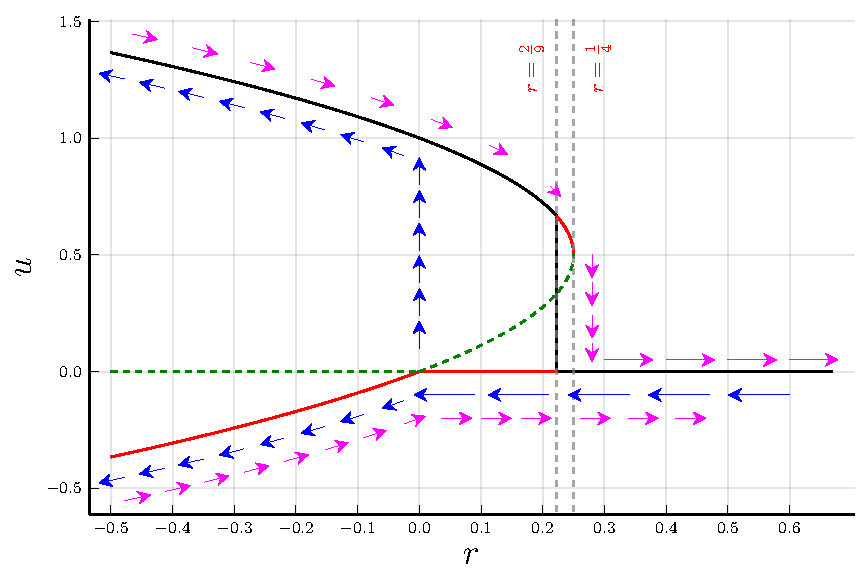
\includegraphics[scale=0.71]{codes/m4hyst.pdf}
    \caption{Hysterisis plot for $\varphi(u)$ with the cubic term. The black line denotes the stable fixed points while the red line represents the metastable fixed points. The dashed green line denote the unstable points.}
    \label{hyst}
\end{figure}
\noindent
So, say if we start from a negative value of $u$ and $r$, then the system quickly moves to the red line (which is locally stable). As we increase $r$, we move along the red line to reach past $r=0$ (shown by the magenta arrows in the lower region of Fig. \ref{hyst}), still following the same line, since the line is locally stable. In this case, there is no hysterisis. \\[0.2cm]
Instead, if we start from some positive value of $u$ initially, the system moves to follow the upper black line; it continues to move like this till $r=\frac{1}{4}$, at which point the line ceases to exist and it quickly drops down to $u=0^+$. \\[0.2cm]
When coming back (starting with a high positive value of $r$), the system remains in $u=0$ line, until $u=0$ becomes unstable at $r=0$. At this point, the system jumps to the globally stable upper black line and continues to move there (shown by the blue lines in the upper part of Fig. \ref{hyst})). \\[0.2cm]
Clearly, these paths, while going and returning, are not the same, and this demonstrates the hysterisis in the theory. 
\subsection{Order Parameter Flow for $m^6$}
Let us move on to the sextic potential that we saw earlier, 
$$\SL = \frac{1}{2}a_2(T-T_c)m^2+\frac{1}{4}a_4m^4 + \frac{1}{6}a_6 m^6 $$
We can perform the same kind of transformation here also. Taking $a_6$ common we have,
$$\SL = a_6\qty (\frac{a_2}{2a_6}(T-T_c)m^2+\frac{a_4}{4a_6}m^4 + \frac{1}{6}m^6) $$
Taking the scaling $a_4 =\pm c^2a_6$ \footnote{If $a_4$ is positive, then we take the $+$ sign, else take the $-$ sign.} and $m=cu$ we obtain,
$$\SL = a_6\qty (\frac{a_2}{2a_6}(T-T_c)c^2u^2\pm \frac{c^6}{4}u^4 + \frac{1}{6}c^6u^6) $$
Defining the new scaling, 
$$\frac{a_2(T-T_c)}{a_6} = rc^4 \implies a_2(T-T_c) = \frac{a_4^2}{a_6}r$$
Taking $c^6$ common and rescaling $\SL$ by $c^6a_6$, we get the transformed function,
\begin{equation}
    \varphi(u) = \frac{1}{2}ru^2 \pm \frac{1}{4}u^4+ \frac{1}{6}u^6
\end{equation}
We do not focus on the case with the $+$ sign. We will deal mainly with the negative coefficient of $u^2$. Minimising $\varphi(u)$ we obtain,
$$ru - u^3 + u^5 = 0 \implies r - u^2+u^4=0$$
which gives us the roots, 
$$u = \pm \sqrt{\frac{1}{2}\pm \sqrt{\frac{1}{4} -r}}\quad \ \ u=0$$
If $r>\frac{1}{4}$, then the only root is $u=0$ (other roots become imaginary). If $0<r<\frac{1}{4}$ then we have all the roots. If $r<0$ then $\sqrt{\frac{1}{4}-r}>\frac{1}{2}$, then there are only three roots, $u=0, \pm \sqrt{\frac{1}{2}+ \sqrt{\frac{1}{4}-r}}$.\\[0.2cm]
Note that $\varphi''(0) = r$ which implies that for $r>0$, $u=0$ is a minima and it is a maxima otherwise. For $r>0$, to check which is the global minima, we check $\varphi(r) = \varphi(0) = 0$ and $\varphi'(u)=0$, which leads to the simultaneous equations, 
\begin{align*}
    6r - 3u^2 + 2u^4&=0\\
    r - u^2 + u^4 &= 0
\end{align*}
solving which, we obtain $u^2 = 4r$ and $r = 0$ or $r = \frac{3}{16}$. Then, for $r>\frac{3}{16}$, $u=0$ is the global minima. For $r<\frac{3}{16}$, $u_{++}$ and $u_{-+}$ are the global stable minimas. Between $\frac{3}{16}<r<\frac{1}{4}$, $u_{++}$ and $u_{-+}$ are the metastable minimas. From this, we obtain the following $u$ vs. $r$ plot. 
\begin{figure}[H]
    \centering 
    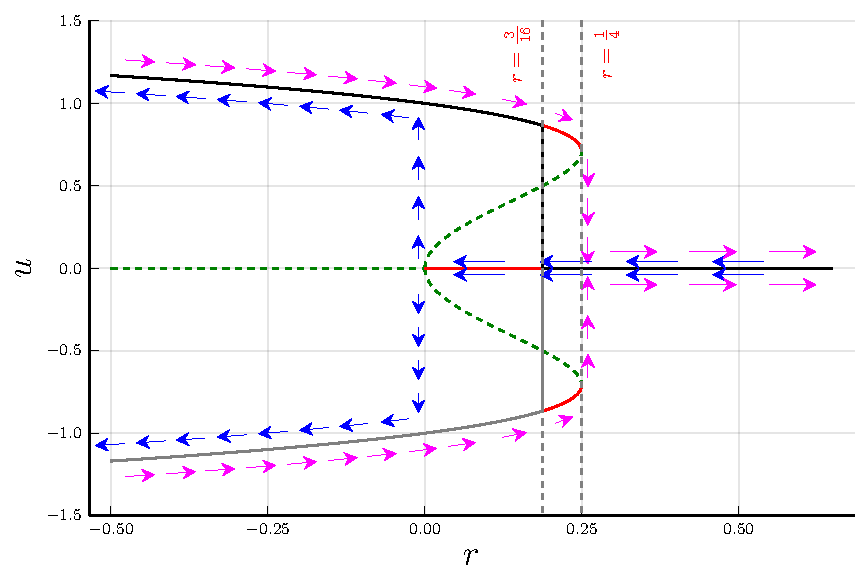
\includegraphics[scale=0.71]{codes/hystm6.pdf}
    \caption{Hysterisis plot for $\varphi(u)$ with $m^6$. The solid black and grey line denote the stable fixed points while the red line represents the metastable fixed points. The dashed green line denote the unstable points.}
    \label{hyst6}
\end{figure}
\noindent
There is an obvious $u\to -u$ symmetry in Fig. \ref{hyst6}. When $r$ is positive, the flow is towards the fixed point $u=0$, which persists even when $r<\frac{1}{4}$. When it reaches $r=0$, $u=0$ becomes unstable and the flow shifts to either of the global fixed points $u_{++}$ or $u_{-+}$.\\[0.2cm] If we instead start from a higher positive value of $u$ when $r<0$, the system shifts to the upper black branch and follows that line till $r=\frac{1}{4}$ where the stable point is annihilated and the system abruptly shifts to $u=0+$, where it remains on increasing $r$ further. We thus see that between $0<r<\frac{1}{4}$, the dynamics is irreversible and there is \textit{hysterisis}. 